\section{Results}
\label{sec:results}

\subsection{Hypotheses}

Hypotheses from the literature:

\begin{itemize}
    \item \textit{"[Humans] overestimate the range of expertise of an automated system and deploy it for tasks at which it is not competent"} \citep[p. 19]{akataResearchAgendaHybrid2020}
    \item \textit{"AI systems [...] were not designed with societal values such as fairness, accountability, and transparency in mind"} \citep[p. 19]{akataResearchAgendaHybrid2020}
\end{itemize}



\subsection{Typical Editorial Process}

The typical editorial process for a manuscript submitted to a scholarly journal looks like the following:

\begin{itemize}
    \item Reviewer reads the manuscript.
    \item Editor makes decision.
\end{itemize}


\subsection{Potential Use Cases For (Hybrid) AI in the Editorial Process}

A simplified, typical editorial process -- from writing to the final decision -- for a manuscript submitted to a scholarly journal is shown in
Figure ~\ref{fig:bpmnEditorialProcess}. The process includes at least three parties: the author who writes the manuscript, the editor of the
journal or conference chair that coordinates the peer-review process, and the peer-reviewers that review and comment on a manuscript. Towards
the end of the writing process, the author will start to think about the journal (or conference) where he/she wants to submit the paper to.
Once the author identified a journal, the manuscript has to be formatted to meet the submission requirements of the journal. 

Table  ~\ref{tab:editorialProcess} shows an overview of the use cases for hybrid AI systems for each step in the typical editorial process.

{\color{purple} @todo: then we can pick those areas where adaptive hybrid AI could be interesting and reason why so\dots}

{\color{purple} @todo: then we can pick exactly one adaptive hybrid AI use case, draw 1-2 hypotheses that we can research 
during the workshop\dots}


\begin{landscape}
    \begin{figure*}[htb]
        \centering
        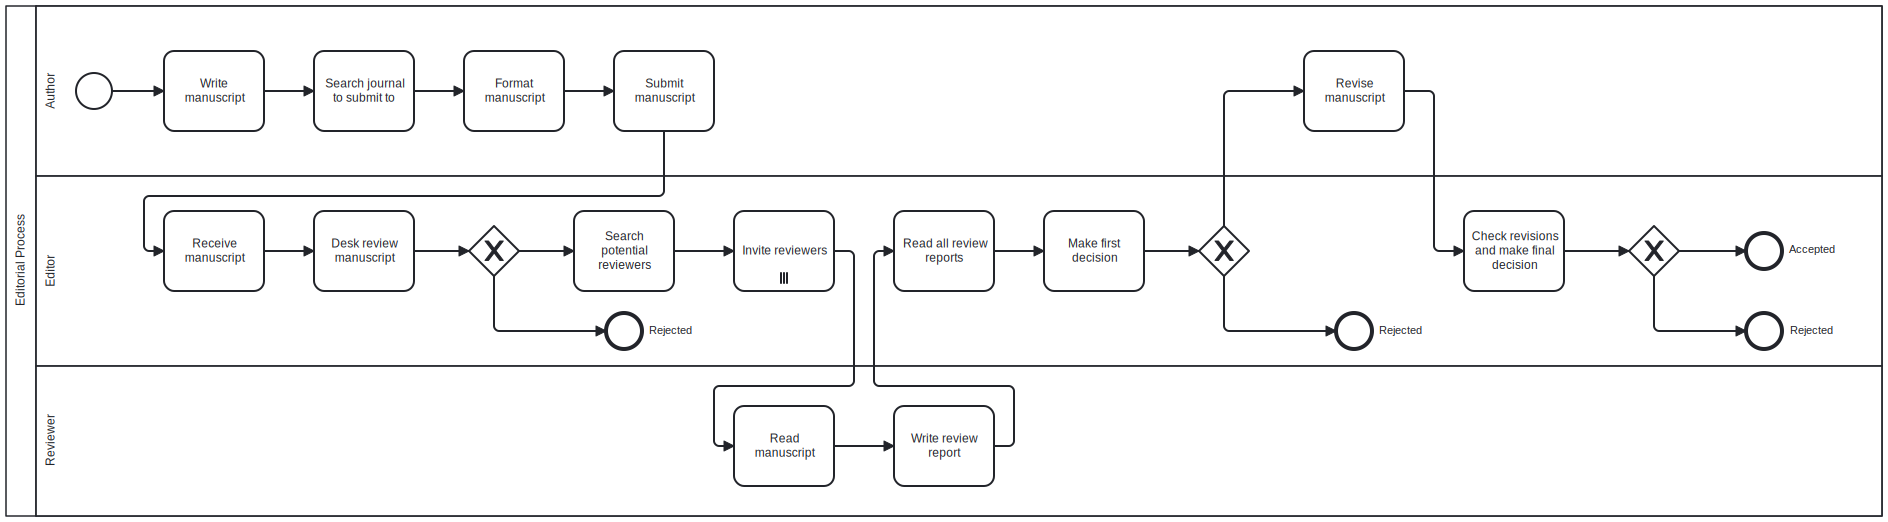
\includegraphics[width=\linewidth]{editorial_process.pdf}
        \caption{A simplified, typical editorial process from writing the manuscript to the final decision of acceptance or
        rejection for publication (in BPMN 2.0). For better understanding, the process steps performed by outside parties 
        are also modelled and the process starts with the outside party (author) writing the manuscript. The numbers
        indicate the sequence flow of the process.}
        \label{fig:bpmnEditorialProcess}
    \end{figure*}

    \begin{table}[htb]
        \caption{Typical editorial processing steps and use cases for (hybrid) AI for a scholarly journal.}
        \label{tab:editorialProcess}
        \renewcommand{\arraystretch}{1.25}
        \small\centering
        \setlength\tabcolsep{6pt}
        \begin{tabularx}{\linewidth}{l l l X}
            \toprule
            \textbf{Step} & \textbf{Role} & \textbf{Task} & \textbf{Use Cases for Hybrid AI} \\
            \midrule

            \circled{1} & Author & Writes manuscript & AI-aided writing, translating, grammar and spell-checking,
                AI-aided literature search and literature review\\

            \circled{2} & Author & Searches for journals to submit to & Decision support system with AI-guided journal recommendation
                based on word embeddings of the manuscript and knowledge engineering using the academic graph\\

            \circled{3} & Author & Formats paper to meet journal's requirements & AI-assisted conversion and formatting of manuscript
                and references, knowledge engineering-based completion of references metadata \\

            \circled{4} & Author & Submits paper to a journal & AI-aided extraction of metadata from the manuscript file \\

            \circled{5} & Editor & Receives manuscript submission & AI-generated summary of the manuscript \\
            
            \circled{6} & Editor & Conducts desk review of the manuscript & Decision support system with AI-assisted checks of the manuscript,
                including detecting plagiarism, tortured phrases ("paraphrased plagiarism"), biased or inappropriate language,
                off-topic references, fabricated or manipulated images, potentially inappropriate authorship, controversial
                topics, etc. Manuscripts are flagged by problem type, ideally by providing examples from within the manuscript,
                for the editor to investigate.\\

            \circled{7} & Editor & Searches for potential reviewers & Decision support system, semantic text similarity search (in vector
                space using document embeddings), graph embeddings, review assignment algorithms using e.g., knowledge graph to 
                exclude potential reviewers with conflicts of interest \\

            \circled{8} & Editor & Invites potential reviewers to review & AI-assisted email writing, AI-generated summary of the manuscript \\

            \circled{9} & Reviewer & Reads the manuscript & AI-assisted summarization of key findings, AI-assisted checking of the content of
                cited references \\

            \circled{10} & Reviewer & Writes review report & AI-assisted writing of qualitative review reports (help reviewer to avoid biases,
                inappropriate feedback, lack of specificity) \\

            \circled{11} & Editor & Reads all review reports & AI-assisted checking of the quality of the peer-review reports \\

            \circled{12} & Editor & Makes decision on manuscript & AI-assisted summarization of peer-review outcome for decision letter
                to author \\

            \circled{13} & Author & Revises manuscript & AI-assisted checking that reviewer concerns are being addressed, AI-assisted
                writing of a rebuttal letter to the reviewers \& editors\\

            \bottomrule
        \end{tabularx}
    \end{table}
\end{landscape}


